\documentclass[a4paper, 12pt]{article}
\usepackage{barinov}
\begin{document}
\thispagestyle{empty}
\begin{center}
    \textit{Федеральное государственное автономное образовательное\\ учреждение высшего образования }

    \vspace{0.5ex}

        \textbf{«Московский физико-технический институт\\ (национальный исследовательский университет)»}
\end{center}

\vspace{10ex}

\begin{center}
    \vspace{13ex}

    \so{\textbf{Лабораторная работа №-.-.-}}

    \vspace{1ex}

    по курсу общей физики

    на тему:

    \textbf{\textit{<<>>}}

    \vspace{30ex}

    \begin{flushright}
        \noindent
        \textit{Работу выполнил:}\\  
        \textit{Баринов Леонид \\(группа Б02-827)}
    \end{flushright}
    \vfill
    Долгопрудный \\2019
\newpage
\setcounter{page}{1}
\fancyhead[R]{\nouppercase{\leftmark}}	
\end{center}

\section{Аннотация}
В работе будет исследовано явление дифракции Френеля и Фраунгофера на
щели, изучено
влияние дифракции на разрешающую способность оптических
инструментов.


\section{Оборудование}
\subsection*{Дифракция Френеля на щели}
Схема установки для наблюдения дифракции Френеля на щели представлена
на рис. 1. Световые лучи освещают щель $S_2$ и испытывают на ней
дифракцию. Дифракционная картина рассматривается с помощью микроскопа
М, сфокусированного на некоторую плоскость наблюдения П.

\begin{figure}[H]
    \includegraphics[width=0.8\linewidth]{1} 
    \captionsetup{justification=centering}
    \caption{Схема установки для наблюдения дифракции Френеля}
\end{figure}

Щель $S_2$ освещается параллельным пучком монохроматического света с
помощью коллиматора, образованного объективом $O_1$, и щелью $S_1$,
находящейся в его фокусе. На щель Si сфокусировано изображение
спектральной линии, выделенной из спектра ртутной лампы Л при помощи
простого монохроматора $C$, в котором используется призма прямого
зрения.

\begin{wrapfigure}{r}{0.3\linewidth}
    \vspace{-16pt}
    \includegraphics[width=\linewidth]{2}
    \captionsetup{justification=centering}
    \caption{Зоны Френеля в плоскости щели}
\end{wrapfigure}

Распределение интенсивности света в плоскости наблюдения П проще всего
рассчитывать с помощью зон Френеля (для щели их иногда называют зонами
Шустера). При освещении щели $S_2$ параллельным пучком лучей (плоская
волна) зоны Френеля представляют собой полоски,
параллельные краям щели (рис. 2). Результирующая амплитуда в точке
наблюдения определяется суперпозицией колебаний от тех зон Френеля,
которые не перекрыты створками щели. Графическое определение
результирующей амплитуды производится с помощью векторной диаграммы —
спирали Корню. Суммарная ширина $m$ зон Френеля $z_m$ определяется
соотношением:
\begin{equation}
    z_m = \sqrt{a m \lambda}
\end{equation}
где $a$ --- расстояние от щели до плоскости наблюдения (рис. 1), а
$\lambda$ --- длина волны.

Вид наблюдаемой дифракционной картины определяется числом Френеля
$\Phi$: квадрат числа Френеля 
\begin{equation}
    \Phi^2 = \frac{D}{\sqrt{a\lambda}}
\end{equation}
--- это отношение ширины щели $D$ к размеру первой зоной Френеля, т.е.
число зон Френеля, которые укладываются на ширине щели. Обратную
величину называют волновым параметром 
\begin{equation}
    p = \frac{1}{\Phi^2} = \frac{\sqrt{a\lambda}}{D}
\end{equation}

Дифракционная картина отсутствует, когда плоскость наблюдения П
совпадает с плоскостью щели: при $\Phi \rightarrow \infty$ мы имеем дело с
геометрической оптикой. При небольшом удалении от щели, когда число
Френеля $\Phi \gg 1$ (на щели укладывается огромное число зон), распределение
интенсивности света за щелью также можно получить с помощью законов
геометрической оптики (приближённо). Дифракционная картина в этом
случае наблюдается только в узкой области на границе света и тени у
краёв экрана.

При последующем небольшом удалении от щели (или изменении ширины щели
$S_2$) эти две группы дифракционных полос перемещаются практически
независимо друг от друга. Каждая из этих групп образует картину
дифракции Френеля на краю экрана. Распределение интенсивности при
дифракции света на краю экрана может быть найдено с помощью спирали
Корню.

При дальнейшем увеличении расстояния а (или уменьшении ширины щели
$S_2$)
обе системы дифракционных полос постепенно сближаются и, наконец, при
$\Phi \gtrsim 1$ накладываются друг на друга. Распределение интенсивности в
плоскости наблюдения в этом случае определяется числом зон Френеля,
укладывающихся на полуширине щели. Если это число равно то, то в поле
зрения наблюдается $n=m-1$ тёмных полос. Таким образом, по виду
дифракционной картины можно оценить число зон Френеля на полуширине
щели.

\subsection*{Дифракция Фраунгофера на щели}

\begin{wrapfigure}[13]{r}{0.3\linewidth}
    \vspace{-10pt}
    \includegraphics[width=\linewidth]{3}
    \caption{К фазовым соотношениям при дифракции Фраунгофера}
\end{wrapfigure}

Картина дифракции резко упрощается, когда ширина щели становится
значительно меньше ширины первой зоны Френеля, т.е. если 
\begin{equation}
    D \ll \sqrt{a \lambda} \quad \text{или} \quad \Phi \ll 1
\end{equation}

Это условие всегда выполняется при достаточно большом расстоянии а от
щели до плоскости наблюдения. Дифракционную картину, наблюдаемую в
этом случае, принято называть дифракцией Фраунгофера. Исследование
такой дифракционной картины заметно облегчается, потому 
что упрощаются фазовые соотношения. Это поясняет рис. 3. При
выполнении условия (4) разность хода между крайними лучами,
приходящими от щели в точку наблюдения $P$, с хорошим приближением можно
вычислять по формуле

\begin{equation}
    \Delta = r_2-r_1 \approx D \sin \Theta \approx D \cdot \Theta
\end{equation}

Здесь предполагается, что дифракционный $\Theta$ достаточно мал, так
что $\sin \Theta \approx \Theta$. Формула (5) справедлива при условии
$\delta \ll \lambda/2$. Можно показать, что это условие эквивалентно
условию (4).

Дифракцию Френеля и Фраунгофера можно наблюдать на одной и той же
установке (рис. 1). Однако при обычных размерах установки дифракция
Фраунгофера возникает только при очень узких щелях. Например, при
$a \approx 20-40\ \text{см}$ и $\lambda \approx 5\cdot 10^{-5}\
\text{см}$ получаем $D \ll 0,3\ \text{мм}$. Поскольку работать с
такими тонкими щелями неудобно, для наблюдения дифракции Фраунгофера к
схеме, изображённой на рис. 1 добавляется объектив $O_2$ (рис. 4).

\begin{figure}[H]
    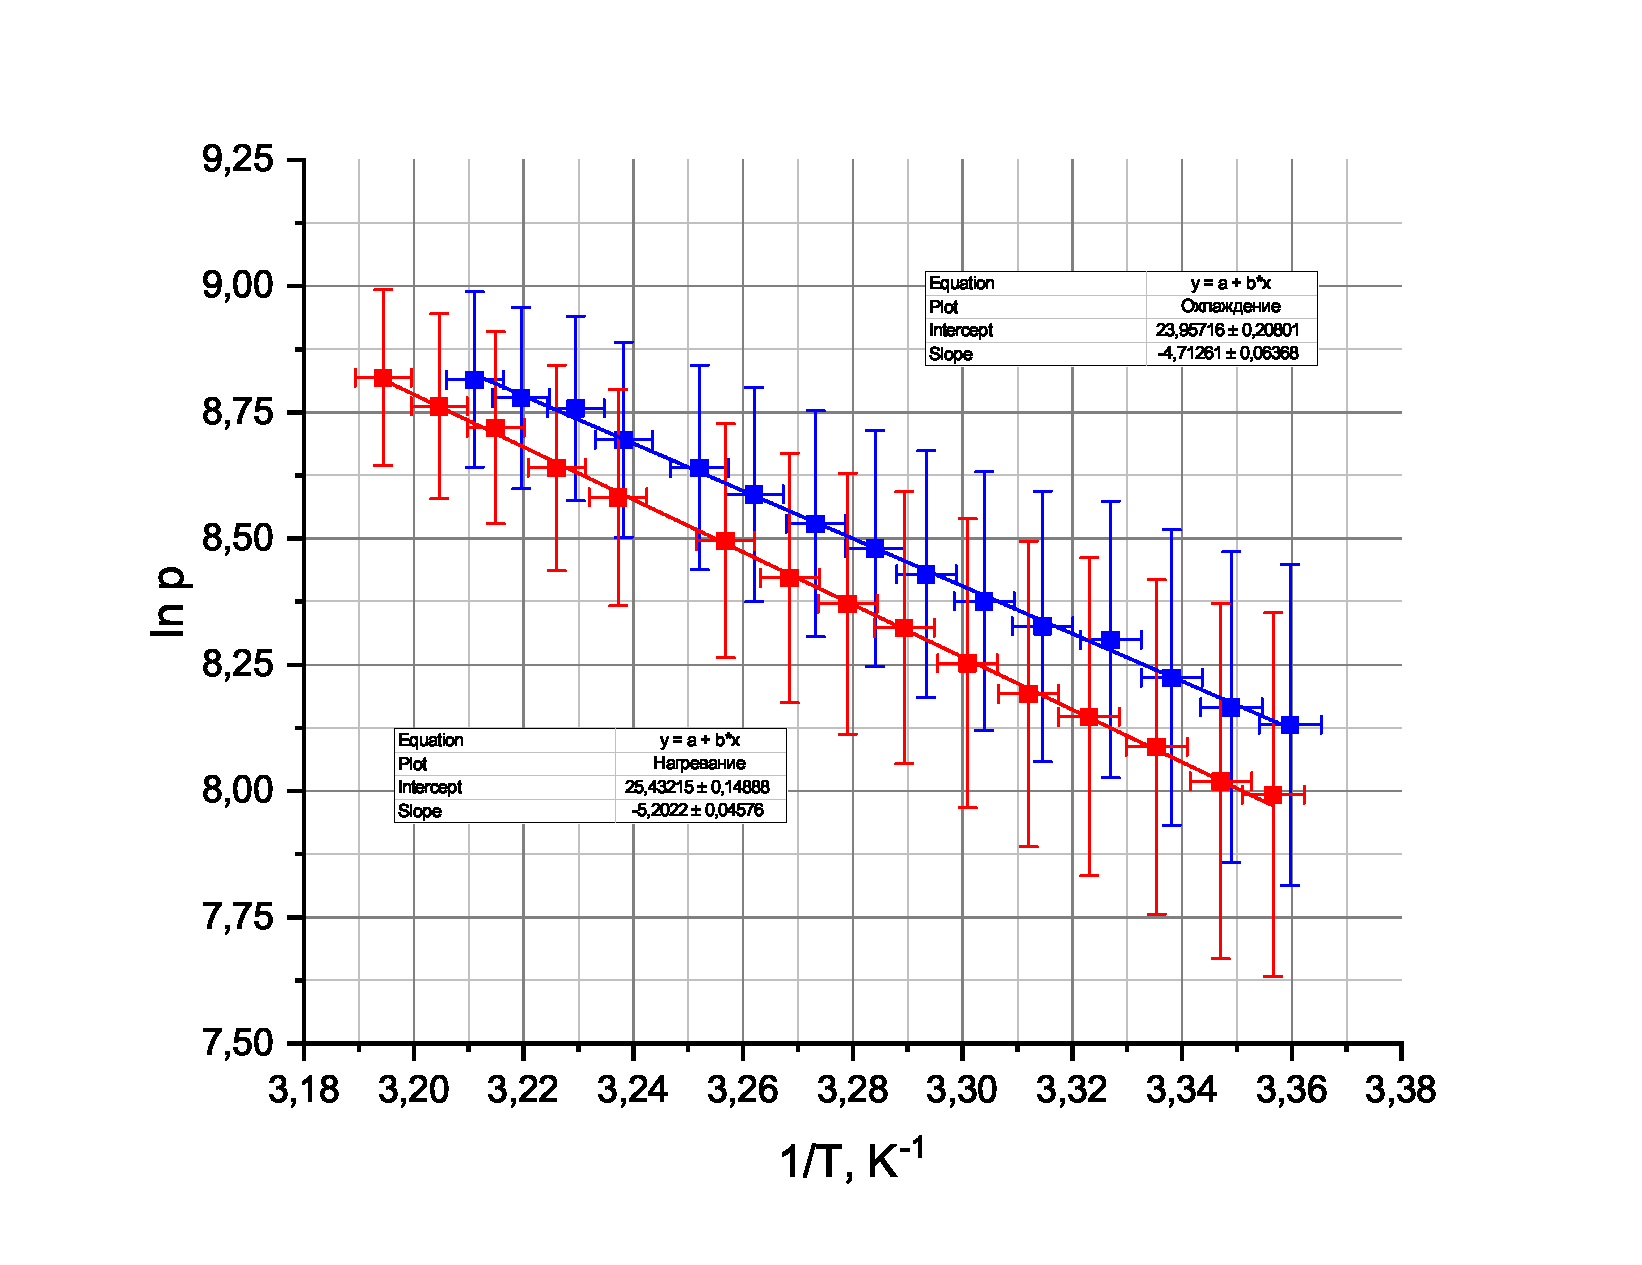
\includegraphics[width=0.8\linewidth]{4} 
    \caption{Схема установки для наблюдения дифракции Фраунгофера на
    щели}
\end{figure}

\begin{wrapfigure}{r}{0.3\linewidth}
    \vspace{-10pt}
    \includegraphics[width=\linewidth]{5}
    \caption{Распределение интенсивности при дифракции Фраунгофера на
    щели}
\end{wrapfigure}

Дифракционная картина наблюдается здесь в фокальной плоскости
объектива $O_2$. Каждому значению угла $\Theta$ соответствует в этой
плоскости точка, отстоящая от оптической оси на расстоянии 
\begin{equation}
    X = f_2 \tg \Theta = f_2 \Theta
\end{equation}

\subsubsection*{Измерение размера выходного зрачка и его удаление}





\section{Результаты измерений и обработка результатов}







\section{Обсуждение результатов и выводы}







\end{document}
